\documentclass[oneside]{emulateapj}
\usepackage{graphicx}				% Use pdf, png, jpg, or eps§ with pdflatex; use eps in DVI mode
								% TeX will automatically convert eps --> pdf in pdflatex	
\usepackage{xcolor}
\usepackage{hyperref}	
\usepackage[sort&compress]{natbib}
\usepackage[hang,flushmargin]{footmisc}
\usepackage[counterclockwise]{rotating}
\newcommand{\teff}{$T_{\rm eff}$ }
\newcommand{\logg}{$\log g$}
\newcommand{\feh}{$\mathrm{[Fe/H]}$}
\newcommand{\vsini}{$v \sin{i}$ }
\newcommand{\tc}{$T_\mathrm{C}$}
\newcommand{\vmacro}{$v_{\mathrm{macro}}$ }
\newcommand{\gcm}{g cm$^{-3}$}
\newcommand{\kms}{km s$^{-1}$}
\newcommand\todo[1]{\textcolor{red}{#1}}  % gotta have \usepackage{xcolor} in main doc or this won't work


\shortauthors{Bedell et al.}
\shorttitle{Kepler-11}

\begin{document}
\graphicspath{ {figures/} }
\DeclareGraphicsExtensions{.pdf,.eps,.png}

\title{Revising the Kepler-11 system: a testament to the importance of precise stellar characterization}

\author{Megan Bedell\altaffilmark{1},
Jacob L. Bean\altaffilmark{1},
Jorge Mel\'{e}ndez\altaffilmark{2},
Sean Mills\altaffilmark{1},
Dan Fabrycky\altaffilmark{1},
Martin Asplund\altaffilmark{3},
Ivan Ram\'{i}rez\altaffilmark{4},
Fan Liu\altaffilmark{3},
David Yong\altaffilmark{3}}

\email{E-mail: mbedell@oddjob.uchicago.edu}

\altaffiltext{1}{Department of Astronomy and Astrophysics, University of Chicago, 5640 S. Ellis Ave, Chicago, IL 60637, USA}
\altaffiltext{2}{Departamento de Astronomia do IAG/USP, Universidade de
S\~{a}o Paulo, Rua do Mat\~{a}o 1226, Cidade Universit\'{a}ria, 05508-900 S\~{a}o Paulo, SP, Brazil}
\altaffiltext{3}{Research School of Astronomy and Astrophysics, The Australian National University, Cotter Road, Weston, ACT 2611, Australia}
\altaffiltext{4}{McDonald Observatory and Department of Astronomy, University of Texas at Austin, USA}

\keywords{stars: abundances, stars: fundamental parameters, techniques: spectroscopic}

\begin{abstract}

The six planets of the Kepler-11 system are the archetypal example of a population of surprisingly low-density transiting planets revealed by the \textit{Kepler} mission. We have determined the stellar chemical composition of Kepler-11 to unprecedented precision using an extremely high quality spectrum from Keck-HIRES (R$\simeq$67000, SNR$\simeq$280). Contrary to previously published results, our spectroscopic constraints indicate that Kepler-11 is a young main-sequence solar twin. The revised stellar parameters raise the densities of the Kepler-11 planets by about 30\%, making them more typical of the emerging class of ``puffy'' close-in exoplanets. We obtain photospheric abundances of 22 elements and find that Kepler-11 is enhanced in refractory materials relative to the solar abundance pattern. We additionally analyze the \textit{Kepler} transits and transit timing variations (TTVs) using a photodynamical model and discuss the tension between spectroscopic and TTV-based stellar density estimates.

\end{abstract}

\section{Introduction}

Five years after their initial discovery, the six planets of the Kepler-11 system remain a crown jewel of \textit{Kepler} science results \citep{Lissauer2011}. All six planets orbit a Sun-like host star at low eccentricies in a largely co-planar, tightly packed configuration. The formation and long-term stability of the system remains an open question \citep[see e.g.][]{Ikoma2012, Hands2014, Mahajan2014}. \todo{say more about resonance, STIPs}

In addition to their unusually tight system architecture, the Kepler-11 planets are noteworthy in another sense: their measured masses and radii place them among the lowest-density super-Earths known to date. Transit timing variations (TTVs) have been measured for all six planets. In the discovery paper, \citet{Lissauer2011} derived mass constraints for the five inner planets based on TTVs from six quarters of \textit{Kepler} data. \citet{Migaszewski2012} reanalyzed the same data using a photodynamical model and found similar results, with an additional constraint on the outermost planet mass. The system was later revisited by \citet{Lissauer2013} using fourteen quarters of \textit{Kepler} data. All three analyses estimate mean densities of $\leq$ 0.5 $\rho_{\earth}$ for all planets in the system, implying a considerable gas envelope on even the smaller super-Earths. This result has considerable repercussions for potential formation system scenarios \todo{(cite)}.

Mean planet densities derived from transits and TTVs (or from transits and radial velocities) have a strong dependence on the properties of the host star. Since the transit depth observationally constrains the ratio of planetary radius to stellar radius, the planet volume depends on the assumed stellar radius to the third power. The planet mass found from TTV inversion is correlated with the stellar mass. Host star characterization is therefore a critical part of measuring planet densities.

In past works, Kepler-11 has been characterized only through spectroscopic analysis of low to modest signal-to-noise data. \citet{Lissauer2011, Lissauer2013, Rowe2014} all use spectra taken by Keck with SNR $\leq$ 40 and apply the Spectroscopy Made Easy package \citep[SME,][]{Valenti1996} to perform matching to a library of synthetic spectra. The resulting stellar atmospheric parameters, when compared with stellar evolution models, indicate that Kepler-11 is a slightly evolved solar analog with (mass, radius). No independent measurements of the stellar density (e.g. from asteroseismology or parallax) are available. Analysis of the stellar composition is also minimal. \citet{Adibekyan2012b} perform an equivalent width (EW) analysis on one of these Keck spectra to derive abundances of three $\alpha$-elements and find that Kepler-11 has moderately low abundances of Ca, Cr, and Ti; however, the line list employed is quite limited with $\leq$ 5 lines per element.

Kepler-11's well-characterized planetary system makes it a prime target for more detailed spectroscopic study. In this work, we present an analysis of a new, very high SNR spectrum. We use equivalent widths to measure the stellar properties and abundances of 22 elements at high precision.


\section{Data}

Owing to its relative faintness (V = 14.2, \citet{Lissauer2011}), Kepler-11 was previously observed only at a signal-to-noise ratio insufficient for high-precision spectroscopic characterization. We dedicated nearly 8 hours of Keck I time to obtaining a higher quality spectrum. Over the course of two consecutive nights (July 26-27 2015), we made 22 1200-s exposures of Kepler-11 for a co-added result of SNR$\simeq$280. For these observations, HIRES was used with the B2 slit and kv387 filter, yielding a resolution R$\simeq$67000 and wavelength coverage between 390 and 830 nm.

We also observed the Sun (using Ceres) and nine bright potential Kepler-11 twins with the same instrumental setup and similar SNR. The Kepler-11 twins were selected by imposing criteria of 5600 $\leq$ \teff$\geq$ 5750 K and 4.2 $\leq$ \logg $\geq$ 4.4 dex on databases of previously published stellar parameters \citep{Adibekyan2012, Bensby2014}. Preference was given to stars likely to be thick-disk members with approximately solar metallicity. These criteria were set based on the original spectroscopic analysis of Kepler-11 by \citet{Lissauer2011}, who found \teff = 5680 $\pm$ 100 K, \logg = 4.3 $\pm$ 0.2 dex, \feh = 0.0 $\pm$ 0.1 dex, and a significant chance of Kepler-11's being a thick disk member based on its kinematics.

The spectral extraction was performed by the Mauna Kea Echelle Extraction (MAKEE) pipeline. All Kepler-11 spectra were then co-added using IRAF's \textit{scombine}.\footnote{IRAF is distributed by the National Optical Astronomy Observatory, which is operated by the Association of Universities for Research in Astronomy (AURA) under cooperative agreement with the National Science Foundation.} Continuum normalization was done by fitting low-order polynomial functions to each order, with care to use the same functional order for a given spectral order on every stellar spectrum to avoid bias in the subsequent differential analysis. Doppler corrections were applied using IRAF's \textit{dopcor} task.

\todo{(details about Kepler lightcurve?)}

\section{Stellar Properties from Spectroscopic Analysis}

The fundamental properties of Kepler-11 and its potential twins were derived from an equivalent width analysis. We hand-measured 94 Fe I and 17 Fe II spectral lines using IRAF's \textit{splot}. The line list was chosen \todo{(criteria, cite)}. Equivalent widths were measured by carefully choosing local continua as described in \citet{Bedell2014} to maximize differential precision between the spectra. The full line list and measured equivalent widths are available in Table \ref{tbl:ews}.

The stellar effective temperature \teff, surface gravity \logg, metallicity \feh, and microturbulence $v_t$ were determined by imposing requirements of excitation and ionization balance on the iron abundances derived by MOOG \citep{Sneden1973}. It is important to note that we exclusively used the differential abundance measurements relative to the solar spectrum. By directly comparing line-by-line differential abundances of spectrally similar stars, we minimize the influence of stellar model systematics on the final parameters and abundances \citep[see e.g.][]{Ramirez2014}. Parameter solutions were found iteratively using the $q^2$ python package.\footnote{\url{https://github.com/astroChasqui/q2}} Uncertainties were determined by propagating scatter among the measured line abundances as described in \citet{Epstein2010, Bensby2014}.

The resulting stellar parameters for all observed stars are given in Table \ref{tbl:param}. The \teff and \logg for Kepler-11 are significantly higher than previously determined values. For example, \citet{Lissauer2013} find \teff = 5666 $\pm$ 60 K, \logg = 4.28 $\pm$ 0.07 dex, and \feh = 0.00 $\pm$ 0.04 dex, while we find \teff = 5839 $\pm$ 7 K, \logg = 4.45 $\pm$ 0.02 dex, and \feh = 0.06 $\pm$ 0.01 dex. Potential sources of this tension include the substantially different SNR of spectra used and the difference in analysis technique. \citet{Lissauer2013} and other previous analyses use SME, which employs a library of synthetic spectra to do spectral matching. 

Our revised stellar parameters securely place Kepler-11 in the solar twin category. This can be seen even by eye: as depicted in Figure \ref{fig:spec}, at high SNR Kepler-11's spectrum is nearly identical to the solar spectrum and distinctly different from that of HD1178, the star from our sample whose fundamental parameters most closely match those found by \citet{Lissauer2013}. In particular, the solar-like \logg for Kepler-11 implies that it is denser and less evolved than previously thought.

We used stellar evolutionary models to estimate the mass, radius, and age of Kepler-11. Yonsei-Yale isochrones were fit using $q^2$. We also applied Dartmouth and Basti isochrones using the \textit{isochrones} python package for fitting. All three models gave results consistent within well below 1$\sigma$. From these fits, we estimate a stellar mass $M_{\star} = 1.04 \pm$ 0.01 $M_{\odot}$, radius $R_{\star} = 1.00 \pm$ 0.02 $R_{\odot}$, and age $2.8 \pm 0.8$ Gyr. This gives a stellar density $\rho_{\star} = 1.47 \pm 0.09$ \gcm.

\begin{figure}
\centering
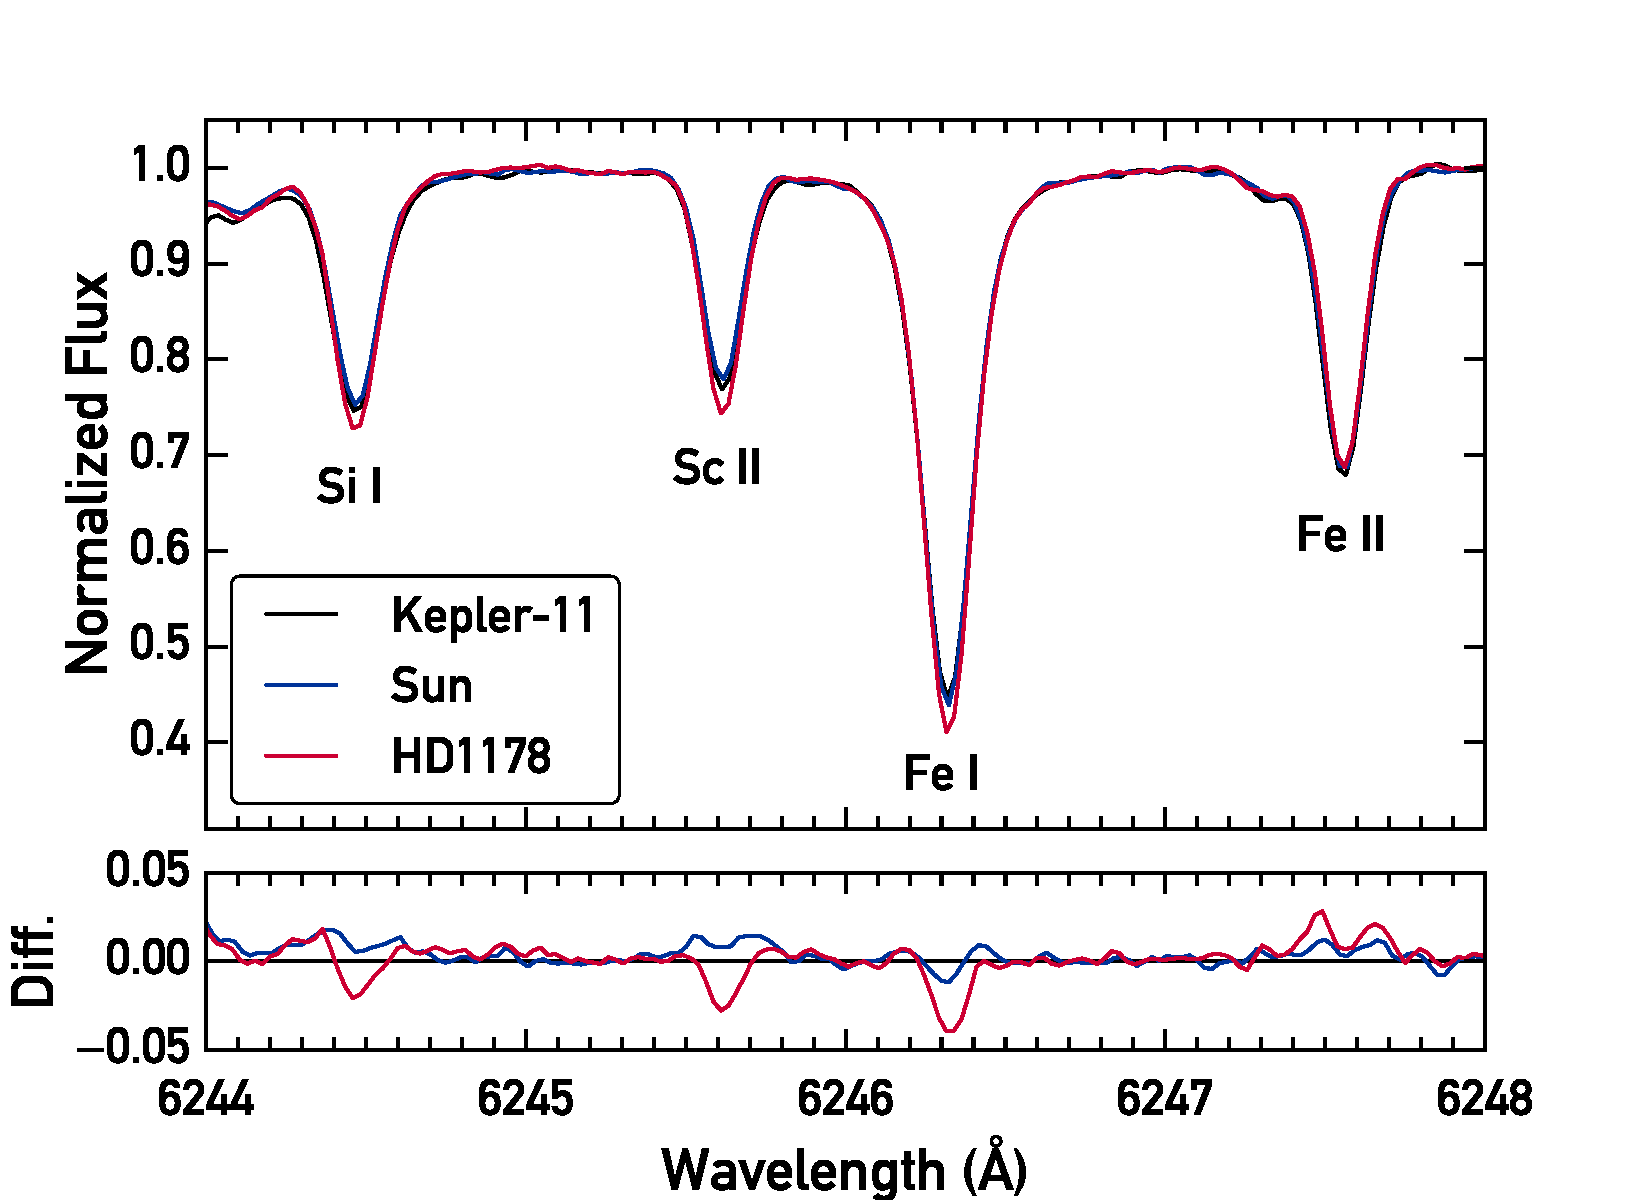
\includegraphics[width=\columnwidth]{spec}
\caption{A small section of the Keck-HIRES spectra of the Sun (blue), Kepler-11 (black), and HD1178 (red), which has fundamental parameters similar to those given by \citet{Lissauer2013} for Kepler-11. Residuals for flux relative to the Kepler-11 spectrum are plotted in the lower panel.}
\label{fig:spec}
\end{figure}

\begin{table*}
\caption{Summary of derived fundamental stellar properties.}
\label{tbl:param}
\centering 
\begin{tabular}{l|cccccccc} 
\hline    
\hline 
{Spectrum}& \teff & $\sigma_{T}$ & \logg & $\sigma_{logg}$ & $v_t$ & $\sigma_{v_t}$ & \feh & $\sigma_{[Fe/H]}$ \\
{}               & (K)           & (K)                 & (dex)     & (dex)                   & (\kms) & (\kms) & (dex) & (dex)  \\
\hline
Sun (Ceres) \footnotemark[1] & 5777 & -- & 4.44 & -- & 0.97 &  -- & 0.0 & -- \\
K11 & 5840 & 7 & 4.46 & 0.02 & 1.00 & 0.02 & 0.063 & 0.007 \\
HD1178 & 5644 & 10 & 4.34 & 0.03 & 0.89 & 0.03 & 0.013 & 0.010 \\
HD10145 & 5627 & 20 & 4.33 & 0.05 & 0.81 & 0.06 & -0.017 & 0.021 \\
HD16623 & 5833 & 47 & 4.51 & 0.09 & 1.07 & 0.10 & -0.434 & 0.034 \\
HD20329 & 5592 & 16 & 4.32 & 0.04 & 0.80 & 0.05 & -0.094 & 0.015 \\
HD21727 & 5608 & 21 & 4.32 & 0.06 & 0.82 & 0.07 & 0.010 & 0.020 \\
HD21774 & 5757 & 27 & 4.33 & 0.06 & 0.99 & 0.06 & 0.251 & 0.024 \\
HD28474 & 5808 & 43 & 4.60 & 0.08 & 1.06 & 0.10 & -0.578 & 0.030 \\
HD176733 & 5597 & 15 & 4.33 & 0.04 & 0.77 & 0.05 & -0.012 & 0.014 \\
HD191069 & 5739 & 29 & 4.33 & 0.09 & 1.03 & 0.08 & -0.029 & 0.025 \\
\hline       
\multicolumn{4}{l}{%
  \begin{minipage}{5.5cm}%
    \footnotetext[1]{Used as reference star.}%
  \end{minipage}%
}\\
\end{tabular}
\end{table*}

\section{Alternative Stellar Age Indicators}

While mass, radius, and density cannot be measured through other methods from the stellar spectrum, stellar age has multiple known proxies. We used several alternate methods to measure the age of Kepler-11 as an independent test of its evolutionary state. The results unanimously agree upon a sub-solar age for Kepler-11. Details of the methods used follow.

\subsection{Stellar Rotation}

The apparent rotation rate \vsini was measured using five saturated lines (Fe I 6027.050 \r{A}, 6151.618 \r{A}, 6165.360 \r{A}, 6705.102 \r{A}, and Ni I 6767.772 \r{A}) from the Keck spectrum. The procedure used is described in depth in \citet{dosSantos2016}, and will be summarized here. We first measured the macroturbulence value \vmacro for each line in the solar reference spectrum with MOOG \textit{synth}. We then calculated \vmacro for Kepler-11 using the measured solar values and the empirical relation given in Equation 1 of \citet{dosSantos2016}. Finally, MOOG \textit{synth} was used to find \vsini for each line in Kepler-11's spectrum with \vmacro fixed to the calculated value.

The five lines give a consistent result of \vsini = 2.2 $\pm$ 0.2 \kms. Assuming alignment of the stellar spin axis with the orbital axis of its transiting planets, we can take \vsini as the true rotational velocity. This translates to an age of \todo{\textbf{x} using \textbf{x}, or \textbf{x}} from \citet{dosSantos2016}'s updated relation.
%Adopting a stellar inclination $i$ = 89.1$^{\circ}$ from \citet{Lissauer2013} and a stellar radius 1.00 \pm$ 0.02 $R_{\odot}$ gives a rotation period of 23 $\pm$ \textbf{x} days.

\subsection{Lithium Abundance}
\label{s:lithium}

The lithium abundance of Kepler-11 was measured by synthesizing the Li I 6707.8 \r{A} line with MOOG \textit{synth}. The line list was adopted from \citet{Melendez2012} and includes blends of atomic and molecular lines. We find a lithium abundance of \textit{A}(Li) = 1.26 $\pm$ 0.05, higher than the solar value of 1.11 at the level of 3$\sigma$ \todo{(Figure \ref{fig:lithium})}. This implies a sub-solar age.

\begin{figure}
\centering
%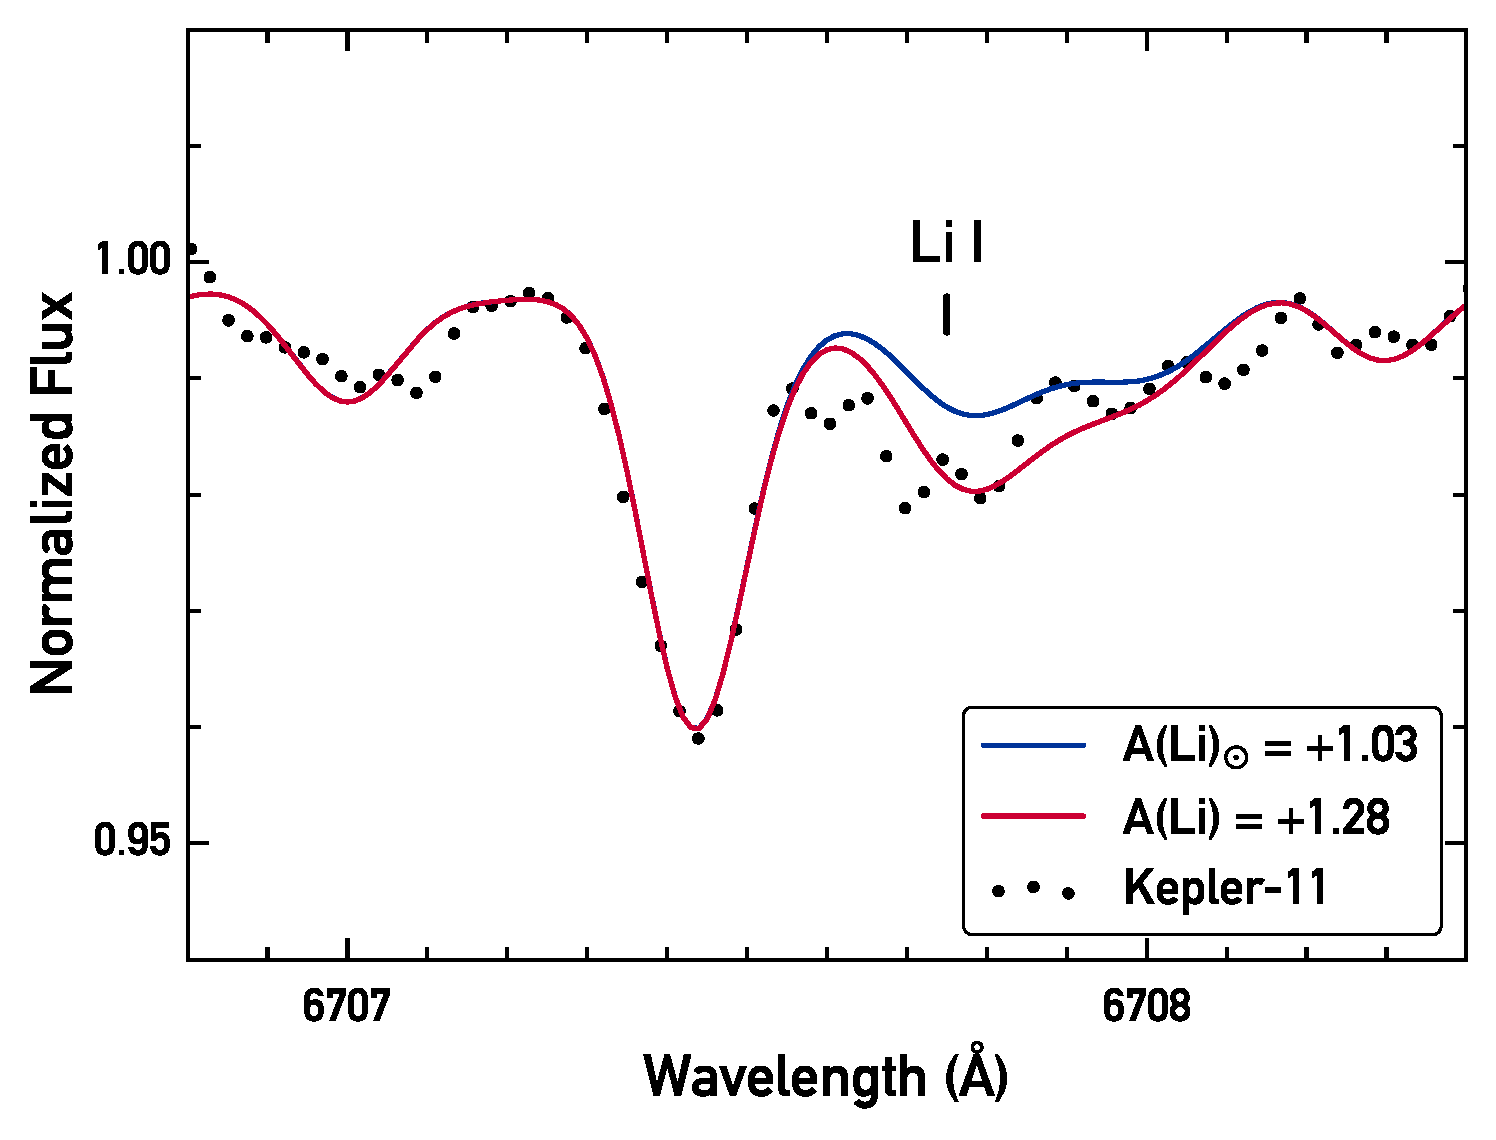
\includegraphics[width=\columnwidth]{lithium}
\caption{Spectra and synthetic fit for Kepler-11 (red) and the Sun (blue) around the Li I 6707.8 \r{A} line.}
\label{fig:lithium}
\end{figure}


\subsection{[Y/Mg] Abundance Ratio}

Recent works by \citet{Nissen2015} and \citet{TucciMaia2016} have identified the ratio of yttrium to magnesium abundances as an excellent proxy for age in main-sequence Sun-like stars. We measured these abundances as described in Section \ref{s:abundances} and found a [Y/Mg] ratio of \todo{\textbf{x}}. Using the age relation from \citet{TucciMaia2016}, this suggests an age of 4.0 $\pm$ 0.7 Gyr.

\subsection{Chromospheric Emission}

We measured the chromospheric emission level of Kepler-11 using the Ca II H\&K lines in the spectrum. \todo{finish}


\section{Stellar Abundances}
\label{s:abundances}

We measured photospheric abundances using the curve-of-growth technique for 20 other elements (excluding lithium, whose synthesis-based abundance determination is discussed in Section \ref{s:lithium}). As with the iron lines, all equivalent widths were measured by hand and line-by-line differential abundances determined with MOOG using $q^2$. The line list was adapted from \todo{(details)}. Hyperfine structure corrections were applied for Co I, Cu I, Mn I, V I, and Y II following \todo{(cite)}. Carbon abundances were measured by a combination of C I and CH lines. Errors on the final abundances were found by adding in quadrature the intrinsic scatter of the lines and the uncertainty propagated from errors on the stellar parameters, as described in \todo{(cite)}. The measured equivalent widths are given in Table \ref{tbl:ews}, and resulting abundances for all stars are in Table \ref{tbl:abund}.

Kepler-11's status as a solar twin enables direct comparison of its abundance pattern to that of the Sun and other known solar twins. Of particular interest is the question of trends in elemental abundances with condensation temperature (\tc). As shown by \citet{Melendez2009}, the solar abundance pattern is unusual in its depletion of refractory elements relative to volatiles. This depletion has been interpreted as ``missing'' rocky material that is locked up in the Solar System planets \citep{Chambers2010}. Building up the number of stars with precisely characterized abundance patterns and planetary systems can help to test this possibility.

We apply corrections for the effects of galactic chemical evolution (GCE), which can change the abundance patterns and \tc trends of stars at varying ages \citep{Nissen2015, Spina2016}. We correct each abundance [X/H] using the prescription of \citet{Spina2016b}, who fit hyperbolic relations to [X/H] as a function of stellar age for a sample of solar twins. We then use the corrected abundances and \tc values from Table 8 of \citet{Lodders2003} to search for a trend. For this part of the analysis, all measured states of a given element (e.g. CI and CH, TiI and TiII, etc.) were combined with a weighted average for the overall elemental abundance. %Although we use differential abundances relative to iron for the fit to be consistent with past literature, we note that the uncertainties used actually correspond to the error on [X/H] rather than [X/Fe]. As noted by \citet{Adibekyan2016}, propagating the iron abundance uncertainty would effectively even out the weighting used in the \tc trend fit. This would be inaccurate since any error in the iron abundance will, to first order, shift all points equally and have no effect on the slope of the \tc trend.

Based on our analysis, Kepler-11 appears to be a ``typical'' solar twin: that is, its abundance pattern is enhanced in refractories relative to the solar pattern (Figure \ref{fig:tc}). The significance of this enhancement depends on the stellar age adopted for the GCE correction. Without GCE correction applied, the \tc slope is significant only at the 2$\sigma$ level, whereas adopting an age of 2.8 Gyr enhances the slope to nearly 5$\sigma$. \todo{(compare to Melendez2009)}

\begin{figure}
\centering
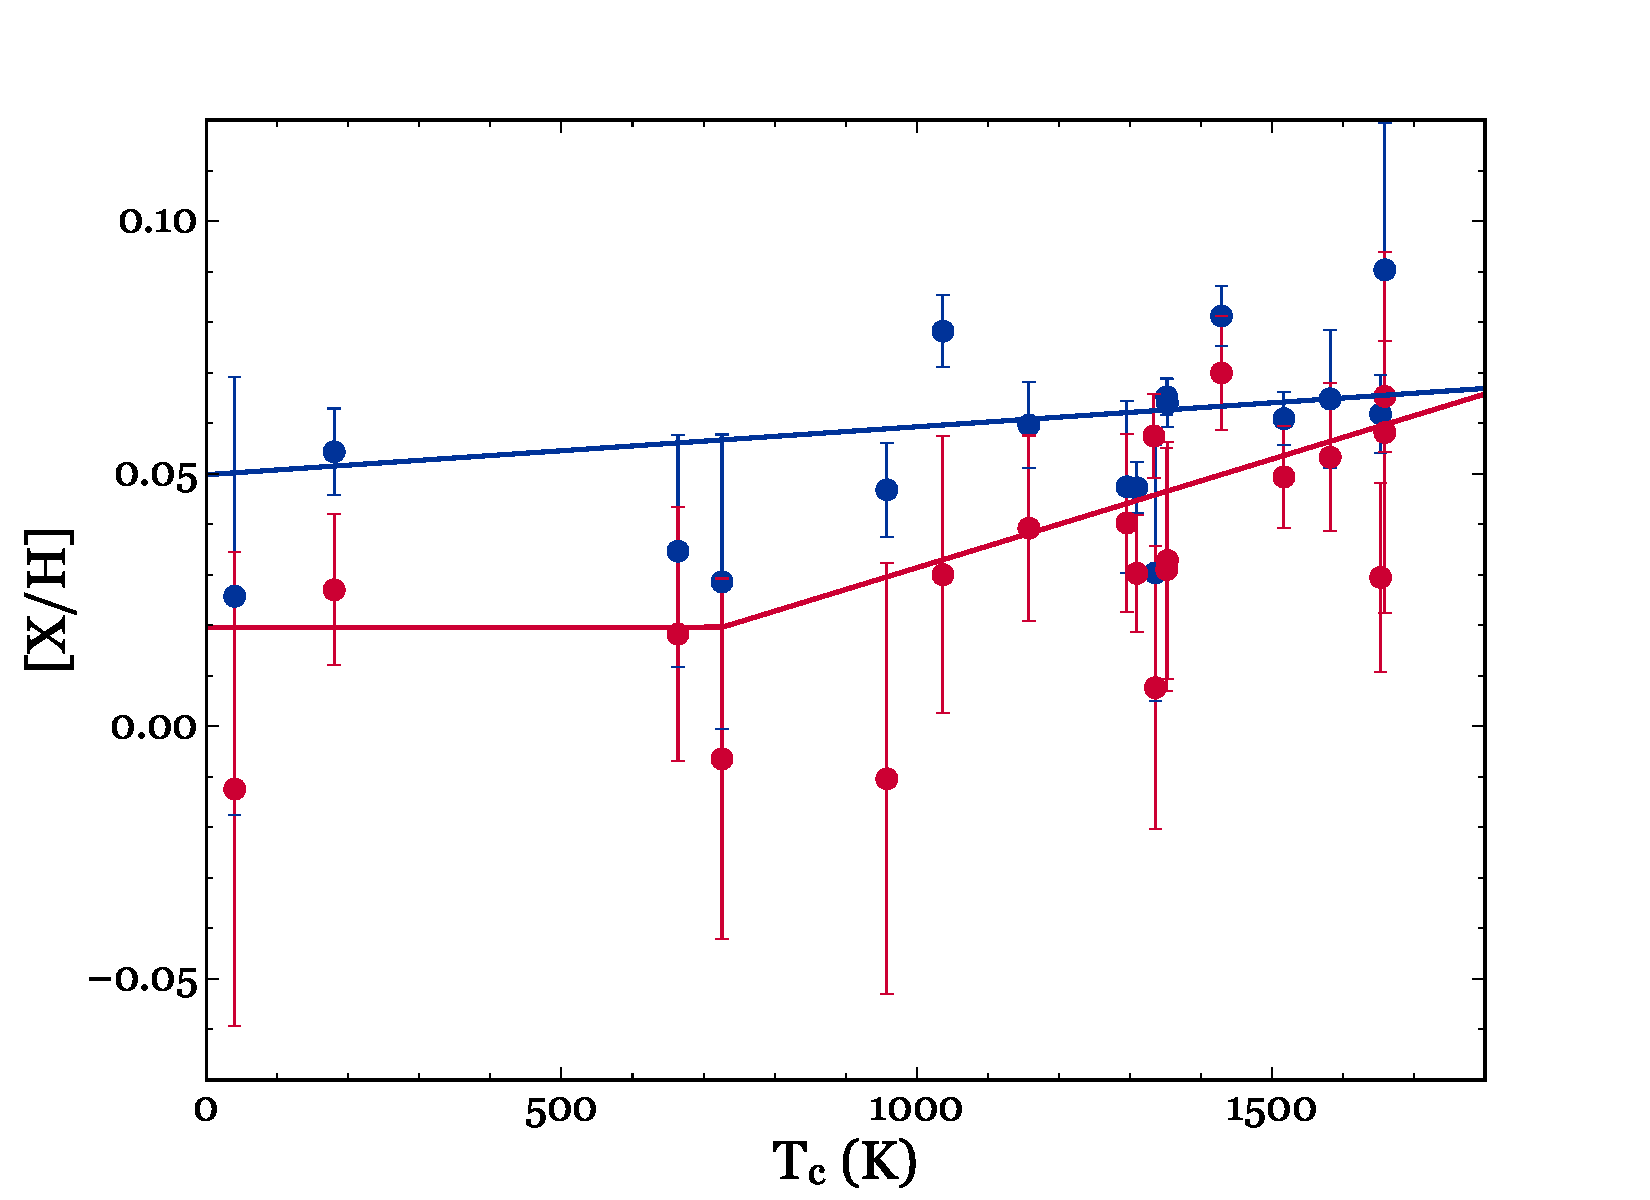
\includegraphics[width=\columnwidth]{K11_Tc_break}
\caption{Differential element abundances of Kepler-11 as a function of the condensation temperature of the element within the protoplanetary disk. The spectral abundances are plotted in blue, and abundances after a GCE correction is applied are in red. \todo{Best-fit models were derived using a }}
\label{fig:tc}
\end{figure}

%***NOTE: add in K abundance and maybe a legend with slope values!



\section{Stellar Properties from Transit \& TTV Analysis}

\section{Discussion}
\subsection{Discrepancies in Stellar Densities}

The stellar densities found through spectroscopic characterization (1.47 $\pm$ 0.09 \gcm) and photodynamical modeling (1.13 $\pm$ 0.07 \gcm) are inconsistent at the level of $\sim$3$\sigma$. While spectroscopically-derived densities can be strongly dependent on imperfect stellar isochrone models, we note that in this case Kepler-11's extreme similarity to the Sun places it near the anchor point of most models, increasing the accuracy of isochronal analysis. Moreover, multiple independent methods support the result of a young, non-evolved age and therefore a solar-like density for Kepler-11.

An alternative hypothesis is that some bias in the transit analysis has resulted in an erroneously low inferred stellar density. As described by \citet{Kipping2014}, multiple effects can bias the density measured by transits, including stellar activity, blended background sources, and non-zero planet eccentricities. \todo{(discuss in detail)}

\subsection{Implications for Planets}

The mass and radius of Kepler-11 has considerable repercussions for its planetary system. We approximate the planet mass derived from TTVs as a linear function of the assumed stellar mass. The planet radius also has a linear dependence on stellar radius, since only the relative surface areas of planet and star can be measured by the transit depth. The stellar properties obtained through spectroscopic analysis therefore raise the planet masses by a factor of 8\% and lower the planet radii by a factor of 6\% relative to the transit and TTV-derived values. The results are shown in Figure \ref{fig:mr}.

Adopting the stellar properties from spectroscopic analysis raises the mean densities of the Kepler-11 planets by $\sim$30\%. This change may go a long way in resolving... \todo{finish}

\begin{figure}
\centering
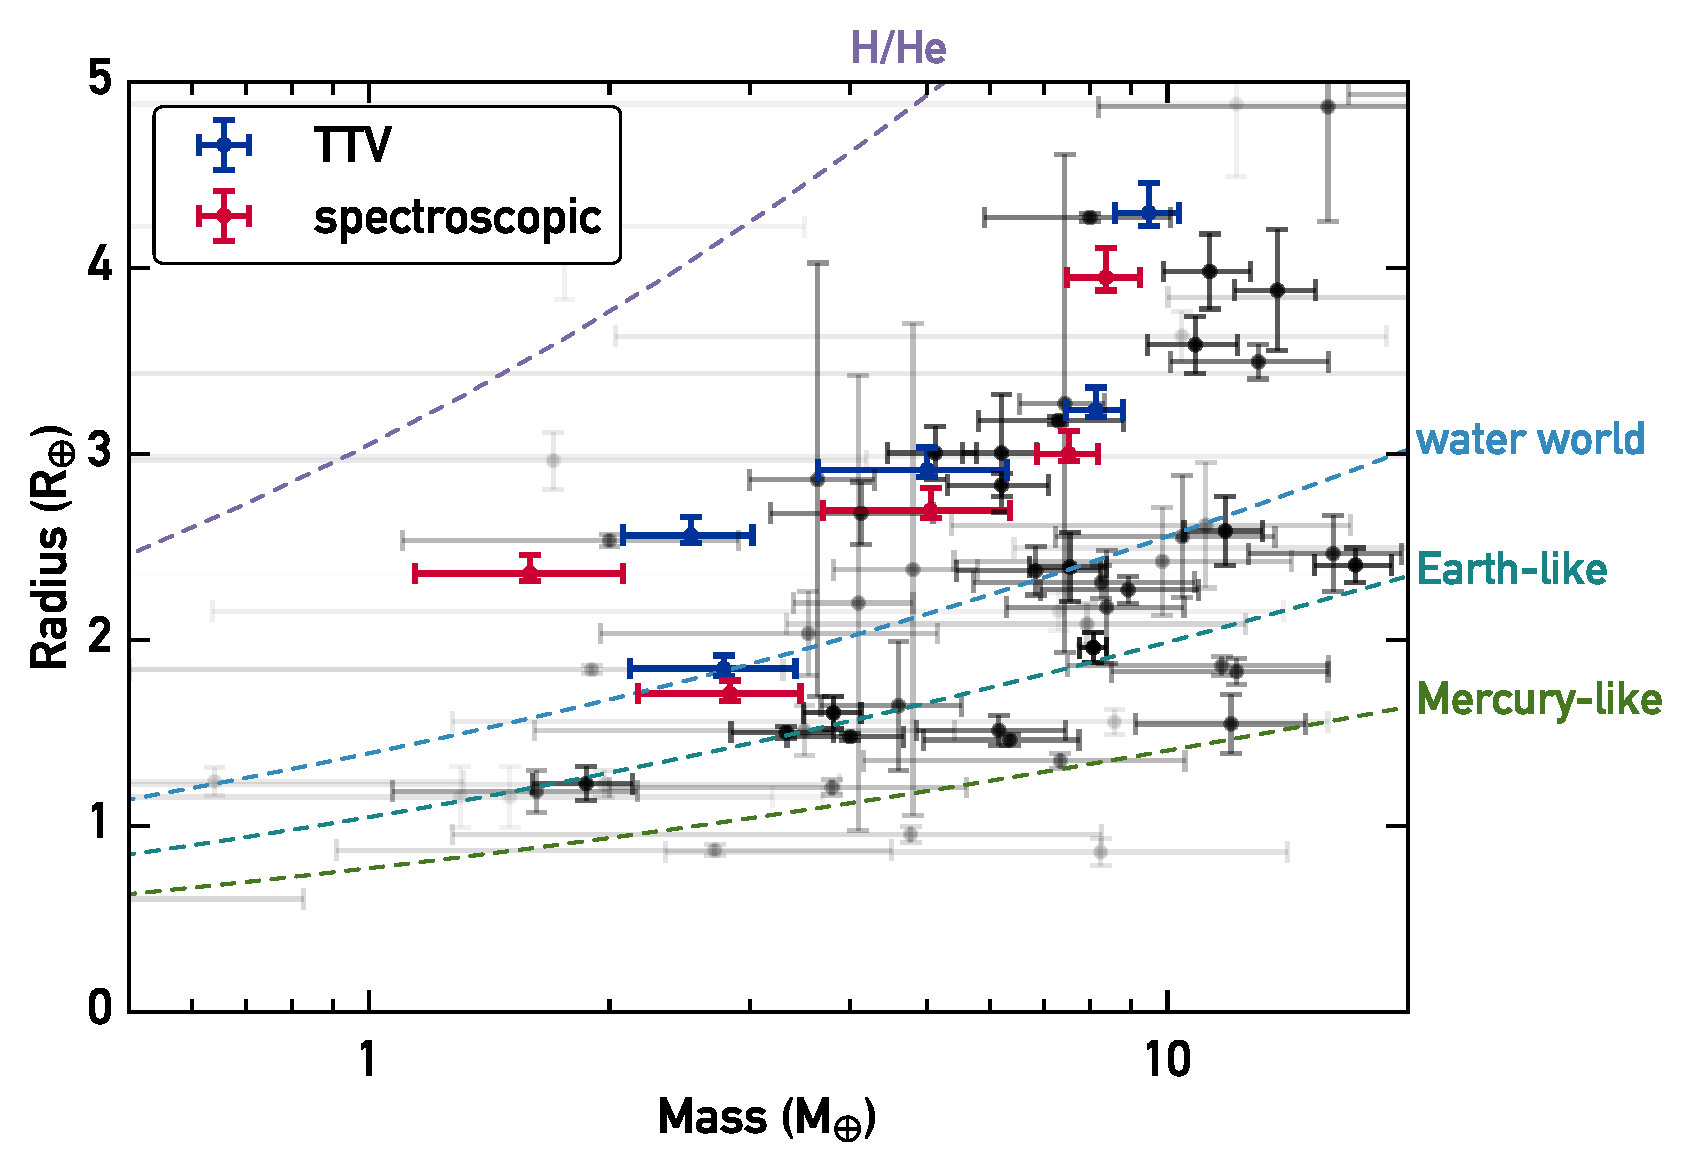
\includegraphics[width=\columnwidth]{K11_massradius}
\caption{Exoplanets with measured masses and radii. Transparencies of the black points scale with the relative error on planet parameters. Kepler-11 a-e are plotted in red (using the transit and TTV-derived parameters) and blue (adjusted by the spectroscopic stellar parameters). Dashed lines show fixed mean densities.}
\label{fig:mr}
\end{figure}


\section{Conclusion}

Using an extremely high-quality spectrum of the multi-planet host star Kepler-11, we have... \todo{finish}

\bigskip
\acknowledgements{M.B. is supported by a National Science Foundation Graduate Research Fellowship under Grant No. DGE-1144082.  J.L.B. acknowledges support for this work from the NSF (grant number AST-1313119) and the Alfred P. Sloan Foundation.  J.M. thanks FAPESP (2012/24392-2). \todo{update \& finish}}

{\it Facilities:} \facility{Keck:I (HIRES)}, \facility{Kepler}


\bibliographystyle{apj}
\bibliography{K11.bib}

\pagebreak
\begin{sidewaystable}
\caption{Line List and Measured Equivalent Widths.}
\label{tbl:ews}
\centering 
\begin{tabular}{cccccccccccccc} 
\hline
\hline
{Wavelength} & Species & EP & log($gf$) & Kepler-11 & HD1178 & HD10145 & HD16623 & HD20329 & HD21727 & HD21774 & HD28474 & HD176733 & HD191069 \\
 (\r{A}) &  & (eV) &  & (m\r{A}) & (m\r{A}) & (m\r{A}) & (m\r{A}) & (m\r{A}) & (m\r{A}) & (m\r{A}) & (m\r{A}) & (m\r{A}) & (m\r{A}) \\
\hline
%  &  & & & & $\vdots$   & &  &  \\
\hline       
\end{tabular}
\tablecomments{Table \ref{tbl:ews} is published in its entirety in the electronic edition of ApJ. A portion is shown here for guidance regarding its form and content.}


\end{sidewaystable}


\pagebreak


\begin{sidewaystable}
\caption{Differential Abundances [X/H].}
\label{tbl:abund}
%\centering 
\begin{tabular}{lccccccccccc} 
\hline    
\hline 
{Element} & $N_{lines}$ & Kepler-11 & HD1178 & HD10145 & HD16623 & HD20329 & HD21727 & HD21774 & HD28474 & HD176733 & HD191069 \\
\hline
CI & 4 & 0.03 $\pm$ 0.01 & 0.12 $\pm$ 0.04 & 0.06 $\pm$ 0.12 & -0.19 $\pm$ 0.08 & 0.05 $\pm$ 0.08 & 0.02 $\pm$ 0.06 & 0.18 $\pm$ 0.04 & -0.07 $\pm$ 0.45 & -0.00 $\pm$ 0.05 & 0.07 $\pm$ 0.03 \\
OI & 3 & 0.05 $\pm$ 0.01 & 0.18 $\pm$ 0.08 & 0.08 $\pm$ 0.02 & -0.08 $\pm$ 0.02 & 0.18 $\pm$ 0.03 & 0.07 $\pm$ 0.03 & 0.20 $\pm$ 0.02 & -0.25 $\pm$ 0.02 & 0.05 $\pm$ 0.03 & 0.14 $\pm$ 0.02 \\
NaI & 4 & 0.05 $\pm$ 0.02 & -0.03 $\pm$ 0.02 & -0.12 $\pm$ 0.05 & -0.37 $\pm$ 0.02 & -0.04 $\pm$ 0.04 & -0.08 $\pm$ 0.03 & 0.27 $\pm$ 0.03 & -0.54 $\pm$ 0.05 & -0.03 $\pm$ 0.03 & -0.01 $\pm$ 0.02 \\
MgI & 5 & 0.03 $\pm$ 0.05 & 0.39 $\pm$ 0.48 & 0.34 $\pm$ 0.48 & -0.07 $\pm$ 0.55 & 0.12 $\pm$ 0.20 & 0.35 $\pm$ 0.47 & 0.36 $\pm$ 0.16 & -0.27 $\pm$ 0.54 & 0.32 $\pm$ 0.48 & 0.35 $\pm$ 0.49 \\
AlI & 2 & 0.06 $\pm$ 0.01 & 0.18 $\pm$ 0.02 & 0.03 $\pm$ 0.00 & -0.28 $\pm$ 0.01 & 0.18 $\pm$ 0.02 & 0.08 $\pm$ 0.00 & 0.28 $\pm$ 0.01 & -0.45 $\pm$ 0.01 & 0.04 $\pm$ 0.00 & 0.11 $\pm$ 0.01 \\
SiI & 14 & 0.05 $\pm$ 0.02 & 0.04 $\pm$ 0.03 & -0.00 $\pm$ 0.01 & -0.27 $\pm$ 0.03 & 0.04 $\pm$ 0.05 & 0.02 $\pm$ 0.03 & 0.25 $\pm$ 0.02 & -0.44 $\pm$ 0.04 & -0.01 $\pm$ 0.02 & 0.04 $\pm$ 0.01 \\
SI & 4 & 0.04 $\pm$ 0.04 & 0.10 $\pm$ 0.04 & 0.05 $\pm$ 0.03 & -0.23 $\pm$ 0.06 & 0.03 $\pm$ 0.09 & 0.01 $\pm$ 0.03 & 0.24 $\pm$ 0.03 & -0.36 $\pm$ 0.09 & 0.02 $\pm$ 0.05 & 0.09 $\pm$ 0.05 \\
KI & 1 & 0.07 $\pm$ 0.00 & 0.07 $\pm$ 0.00 & 0.02 $\pm$ 0.00 & -0.22 $\pm$ 0.00 & 0.03 $\pm$ 0.00 & 0.01 $\pm$ 0.00 & 0.15 $\pm$ 0.00 & -0.42 $\pm$ 0.00 & -0.00 $\pm$ 0.00 & 0.08 $\pm$ 0.00 \\
CaI & 11 & 0.06 $\pm$ 0.02 & 0.02 $\pm$ 0.14 & -0.05 $\pm$ 0.17 & -0.28 $\pm$ 0.05 & 0.18 $\pm$ 0.24 & 0.04 $\pm$ 0.15 & 0.19 $\pm$ 0.08 & -0.47 $\pm$ 0.06 & -0.07 $\pm$ 0.20 & 0.04 $\pm$ 0.03 \\
ScI & 4 & 0.09 $\pm$ 0.04 & 0.09 $\pm$ 0.03 & 0.02 $\pm$ 0.03 & -0.30 $\pm$ 0.06 & 0.06 $\pm$ 0.06 & 0.03 $\pm$ 0.03 & 0.27 $\pm$ 0.03 & -0.33 $\pm$ 0.08 & -0.01 $\pm$ 0.04 & 0.08 $\pm$ 0.01 \\
ScII & 5 & 0.09 $\pm$ 0.02 & 0.14 $\pm$ 0.06 & 0.03 $\pm$ 0.02 & -0.24 $\pm$ 0.04 & 0.14 $\pm$ 0.06 & 0.10 $\pm$ 0.05 & 0.32 $\pm$ 0.02 & -0.41 $\pm$ 0.05 & -0.00 $\pm$ 0.02 & 0.12 $\pm$ 0.04 \\
TiI & 18 & 0.07 $\pm$ 0.02 & 0.12 $\pm$ 0.03 & 0.05 $\pm$ 0.05 & -0.21 $\pm$ 0.04 & 0.15 $\pm$ 0.03 & 0.07 $\pm$ 0.04 & 0.24 $\pm$ 0.04 & -0.41 $\pm$ 0.03 & 0.02 $\pm$ 0.03 & 0.08 $\pm$ 0.02 \\
TiII & 11 & 0.07 $\pm$ 0.03 & 0.11 $\pm$ 0.05 & 0.01 $\pm$ 0.09 & -0.18 $\pm$ 0.05 & 0.11 $\pm$ 0.03 & 0.01 $\pm$ 0.10 & 0.26 $\pm$ 0.04 & -0.37 $\pm$ 0.04 & -0.02 $\pm$ 0.03 & 0.11 $\pm$ 0.04 \\
VI & 9 & 0.08 $\pm$ 0.02 & 0.07 $\pm$ 0.02 & -0.02 $\pm$ 0.03 & -0.28 $\pm$ 0.03 & 0.08 $\pm$ 0.09 & 0.04 $\pm$ 0.03 & 0.28 $\pm$ 0.02 & -0.48 $\pm$ 0.04 & -0.00 $\pm$ 0.02 & 0.04 $\pm$ 0.02 \\
CrI & 10 & 0.04 $\pm$ 0.02 & 0.02 $\pm$ 0.03 & 0.01 $\pm$ 0.07 & -0.47 $\pm$ 0.03 & -0.06 $\pm$ 0.03 & 0.02 $\pm$ 0.03 & 0.27 $\pm$ 0.03 & -0.60 $\pm$ 0.06 & 0.01 $\pm$ 0.03 & -0.02 $\pm$ 0.02 \\
CrII & 5 & 0.05 $\pm$ 0.02 & 0.01 $\pm$ 0.02 & -0.02 $\pm$ 0.05 & -0.38 $\pm$ 0.06 & -0.08 $\pm$ 0.02 & 0.01 $\pm$ 0.03 & 0.24 $\pm$ 0.03 & -0.55 $\pm$ 0.05 & -0.03 $\pm$ 0.04 & -0.02 $\pm$ 0.02 \\
MnI & 8 & 0.06 $\pm$ 0.02 & -0.04 $\pm$ 0.03 & -0.07 $\pm$ 0.04 & -0.61 $\pm$ 0.02 & -0.18 $\pm$ 0.02 & -0.04 $\pm$ 0.03 & 0.30 $\pm$ 0.03 & -0.75 $\pm$ 0.06 & -0.02 $\pm$ 0.03 & -0.08 $\pm$ 0.02 \\
FeI & 92 & 0.06 $\pm$ 0.03 & 0.02 $\pm$ 0.04 & -0.02 $\pm$ 0.06 & -0.43 $\pm$ 0.09 & -0.09 $\pm$ 0.05 & 0.01 $\pm$ 0.08 & 0.25 $\pm$ 0.08 & -0.58 $\pm$ 0.08 & -0.01 $\pm$ 0.05 & -0.03 $\pm$ 0.09 \\
FeII & 17 & 0.06 $\pm$ 0.02 & 0.02 $\pm$ 0.05 & -0.02 $\pm$ 0.11 & -0.43 $\pm$ 0.07 & -0.10 $\pm$ 0.05 & 0.00 $\pm$ 0.04 & 0.25 $\pm$ 0.03 & -0.58 $\pm$ 0.07 & -0.02 $\pm$ 0.03 & -0.03 $\pm$ 0.04 \\
CoI & 6 & 0.07 $\pm$ 0.01 & 0.05 $\pm$ 0.04 & -0.04 $\pm$ 0.03 & -0.27 $\pm$ 0.04 & 0.01 $\pm$ 0.03 & -0.01 $\pm$ 0.03 & 0.26 $\pm$ 0.01 & -0.45 $\pm$ 0.03 & -0.02 $\pm$ 0.01 & 0.06 $\pm$ 0.02 \\
NiI & 20 & 0.06 $\pm$ 0.02 & 0.00 $\pm$ 0.07 & -0.03 $\pm$ 0.03 & -0.42 $\pm$ 0.03 & -0.05 $\pm$ 0.04 & 0.01 $\pm$ 0.05 & 0.31 $\pm$ 0.16 & -0.60 $\pm$ 0.03 & 0.00 $\pm$ 0.05 & -0.01 $\pm$ 0.02 \\
CuI & 4 & 0.08 $\pm$ 0.01 & 0.08 $\pm$ 0.03 & -0.02 $\pm$ 0.02 & -0.44 $\pm$ 0.05 & 0.00 $\pm$ 0.01 & -0.00 $\pm$ 0.02 & 0.32 $\pm$ 0.03 & -0.59 $\pm$ 0.09 & 0.06 $\pm$ 0.03 & 0.06 $\pm$ 0.02 \\
ZnI & 3 & 0.03 $\pm$ 0.04 & 0.05 $\pm$ 0.02 & 0.01 $\pm$ 0.04 & -0.31 $\pm$ 0.06 & 0.07 $\pm$ 0.02 & -0.00 $\pm$ 0.03 & 0.28 $\pm$ 0.05 & -0.52 $\pm$ 0.09 & 0.00 $\pm$ 0.02 & 0.08 $\pm$ 0.02 \\
YII & 5 & 0.07 $\pm$ 0.02 & -0.01 $\pm$ 0.01 & -0.05 $\pm$ 0.03 & -0.52 $\pm$ 0.03 & -0.12 $\pm$ 0.03 & -0.04 $\pm$ 0.02 & 0.23 $\pm$ 0.01 & -0.61 $\pm$ 0.04 & -0.04 $\pm$ 0.03 & -0.08 $\pm$ 0.01 \\
CH & 3 & 0.03 $\pm$ 0.05 & 0.03 $\pm$ 0.12 & -0.04 $\pm$ 0.13 & -0.45 $\pm$ 0.11 & -0.17 $\pm$ 0.09 & -0.05 $\pm$ 0.09 & 0.24 $\pm$ 0.05 & -0.65 $\pm$ 0.14 & -0.08 $\pm$ 0.29 & 0.04 $\pm$ 0.08 \\
\hline       
\end{tabular}
\end{sidewaystable}





\end{document}  